\newpage
\section{Simulation Analysis}
\label{sec:simulation}
Since the input voltage source in this circuit is sinusoidal, the voltage and current values of the various components vary in time, and we are interested therefore in analysing how they evolve in time and obviously we want to picture the transformation of our AC input voltage source throughout the multiple stages of the circuit. We will run an operating point analysis in order to confirm the forward-active region of the two transisters, a transient analysis which will help us measuring the input and output impedances. We will also run a frequency response analysis in order to determine the gain and bandwidth of our output amplified sinusoidal signal. The transistors used were the Philips BJT's.

\subsection{Operating point}
We start with the operating point analysis. Given that the output signal will be solely sinusoidal, there isn't much relevance to this set of data. Its main goal is to confirm the forward-active region of both the npn and pnp transistors. In table~\ref{tab:operator} we present the operating point node voltages of the circuit. As expected, the voltage in nodes $in$ e $in2$ since our source doesn't have a DC component. Our output signal doesn't have a linear voltage component, since the voltage in node $out$ is zero, because the output coupling capacitor blocks the coming DC voltage. Regarding the npn transistor, the voltage drop must occur from the collector to the base, and from the base to the emitter - since $V_{coll}>V_{base}>V_{emit}$, this is confirmed. Looking to the pnp transistor, our collector node is ground, our base node is $coll$ and our emitter node is $emit2$. The voltage drop in this case must happen from the emitter to the collector. Since $V_{emit2}>V_{coll}>GND$, this is confirmed - both our transistors work in the pretended forward-active region.

\begin{table}[h]
  \centering
  \begin{tabular}{|l|r|}
    \hline    
    {\bf Name} & {\bf Values [V]} \\ \hline
    @gb[i] & -2.29771e-04\\ \hline
@idd[current] & 1.005042e-03\\ \hline
@r1[i] & 2.191669e-04\\ \hline
@r2[i] & 2.297712e-04\\ \hline
@r3[i] & 1.060424e-05\\ \hline
@r4[i] & 1.185502e-03\\ \hline
@r5[i] & 1.234813e-03\\ \hline
@r6[i] & 9.663347e-04\\ \hline
@r7[i] & 9.663347e-04\\ \hline
v(1) & -9.73914e-01\\ \hline
v(3) & 1.063433e+01\\ \hline
v(4) & 6.382611e+00\\ \hline
v(5) & 6.843347e+00\\ \hline
v(6) & 7.067298e+00\\ \hline
v(7) & 1.953900e+00\\ \hline
v(8) & 6.875344e+00\\ \hline
v(9) & 0.000000e+00\\ \hline
 
  \end{tabular}
  \caption{Operating point node voltage values of the amplifier circuit.}
  \label{tab:operator}
\end{table}

\subsection{Frequency response and impedances}
We measured the input impedance of the circuit, seen through the perspective of the source, and the output impedance, seen through the perspective of our output (using a dummy test source). With the frequency response, we measured the voltage gain in our output. As we will see in figure~\ref{fig:outputstage}, the gain graph has the traits of a band-pass filter, letting pass medium frequencies (our source operates at a medium frequency), so we measure the in that zone. We also measured then the lower and upper cut-off frequencies of such graph, in order to determine the bandwidth of our amplifier. In table~\ref{tab:main}, we present the results of our calculations. In figures~\ref{fig:gainstage}and~\ref{fig:outputstage} we can see the evolution of the gain throughout the circuit, first the gain out of the gain stage - node $coll$ - and then the final gain, the gain out of the output stage - node $out$. With this figures we can confirm the band-pass filter trait of our circuit.

\begin{table}[h]
  \centering
  \begin{tabular}{|l|r|}
    \hline    
    {\bf Name} & {\bf Values} \\ \hline
    @$V_{DC}$ & 12.000000 \\ \hline 
@$V_{ACripple}$ & 0.000015 \\ \hline 
Cost & 1902.400000 \\ \hline 
Merit & 33.573648 \\ \hline 

    \input{outimp_tab}     
  \end{tabular}
  \caption{Output gain, bandwidth, and input and output impedances of the audio amplifier circuit (as a whole).}
  \label{tab:main}
\end{table}

Analysing both the input and output impedances of the circuit, the input impedance is pretty satisfactory as it allows the vast majority of input voltage to go through the transistors, which means a low voltage loss. However, comparing the value of the output impedance with the load resistor, they are very much comparable. This means that part of the gain coming from the transistors will be consumed by some of our resistors in the circuit, hence losing a considerable part of the possible output gain. However, given the gain value we obtained, the overall result is very satisfying.

\begin{figure}[!h] \centering
\includegraphics[width=0.6\linewidth]{stage.pdf}
\caption{Gain Stage output voltage gain (frequency response).}
\label{fig:gainstage}
\end{figure}

\begin{figure}[!h] \centering
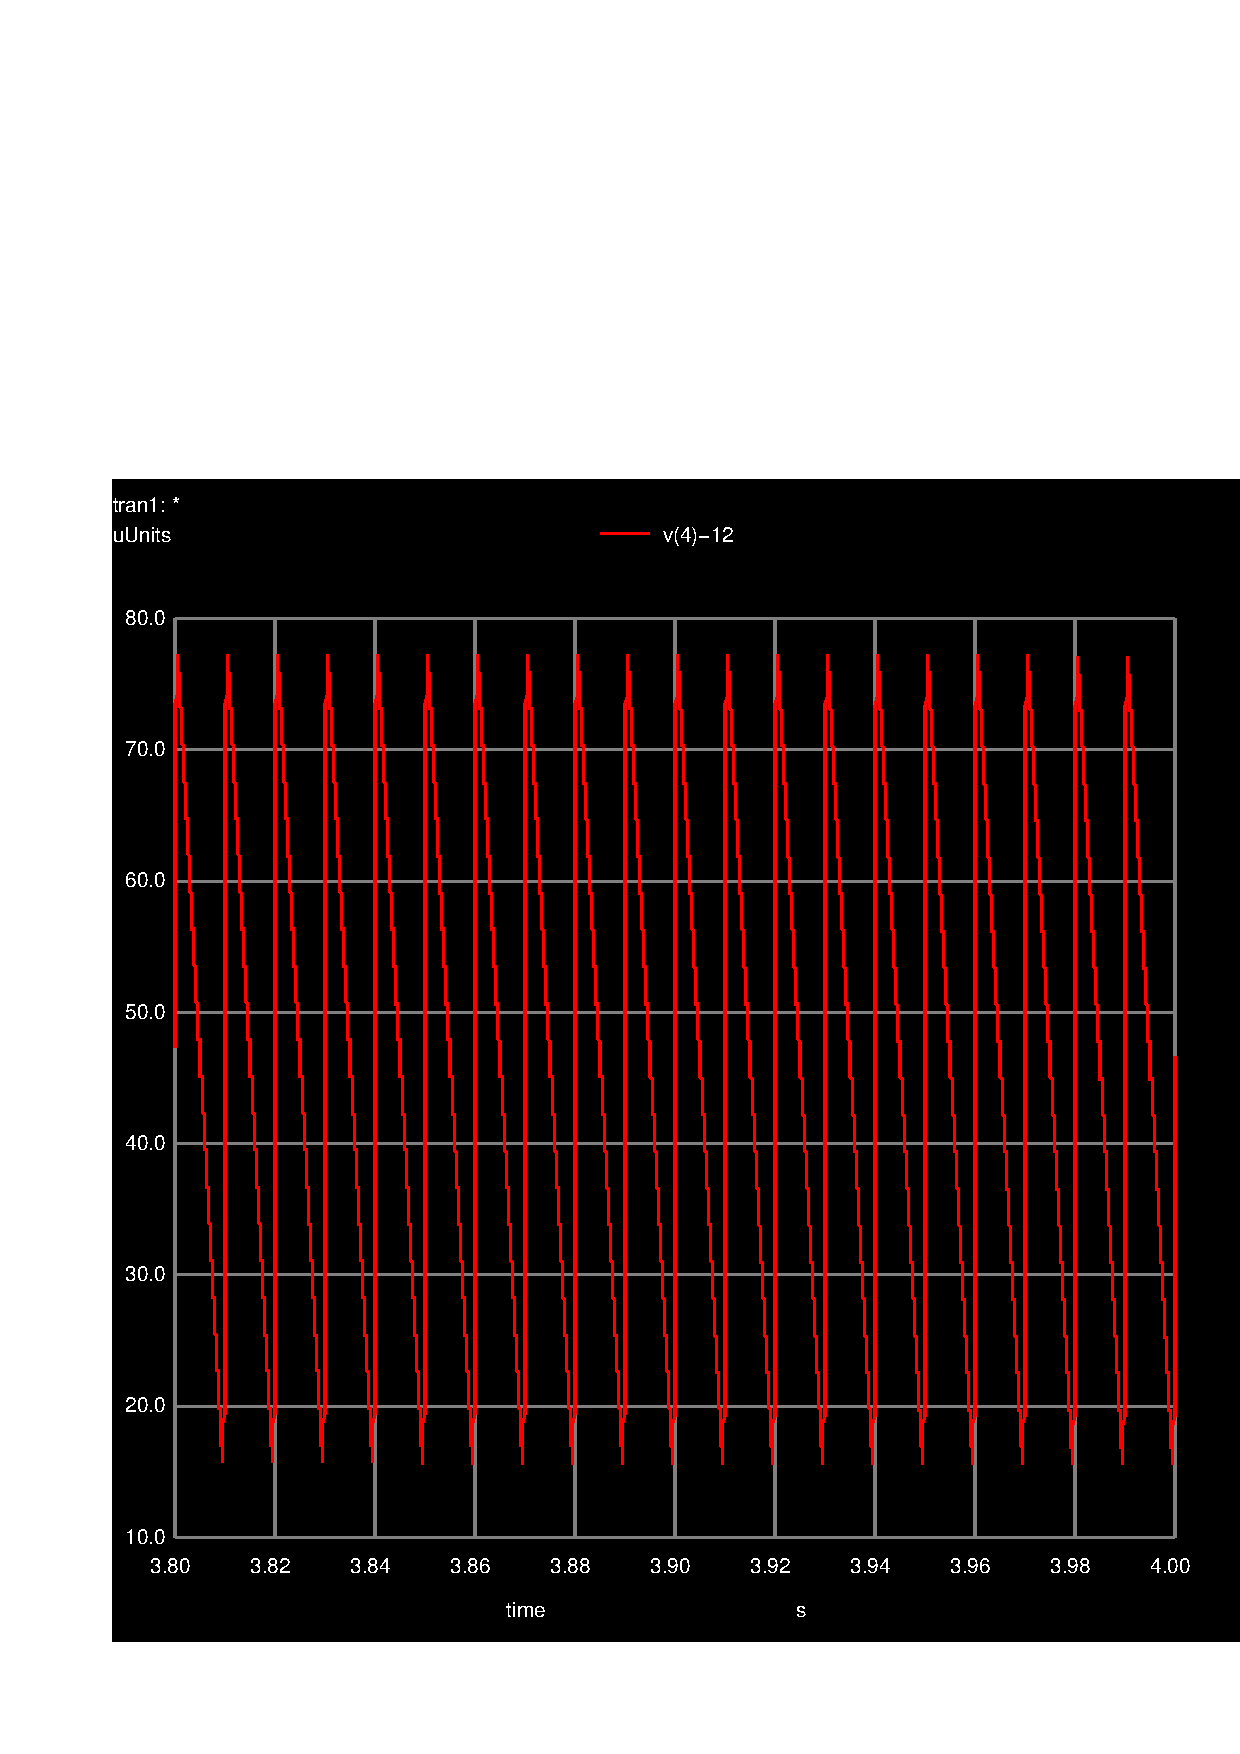
\includegraphics[width=0.6\linewidth]{output.pdf}
\caption{Load output voltage gain (frequency response).}
\label{fig:outputstage}
\end{figure}

\subsection{Final product and merit}
In figure~\ref{fig:comp}, we can see the evolution of our AC signal from stage to stage until its final form. The output voltage has a null DC component as pretended, a symmetric phase in comparison to the input source (it's inverted) and a clear greater amplitude of approximately 0.55V, in comparison to the input's 10mV. We can say then that we have achieved the goal of amplifying our input signal, in this case, by 50-60 times!
In table~\ref{tab:merit}, we present the cost and merit of our circuit. When looking to the parameters judged by the merit formula, we achieved an amazing bandwidth that clearly operates in the 20Hz-20kHz frequency band pretended, since we have an upper cut-off frequency in the zone of MHz, and a lower cut-off frequency inferior to 20Hz - $\approx$16Hz. The voltage gain could always be a bit higher, but without a defined pretended output amplitude, we can't really evaluate our achieved gain. Since we achieved a merit similar to 2326, the high cost seems like a reasonable price to pay for a circuit with these results. We were able however to achieve greater values of gain, but the output sinusoidal wave would be distorted, almost "cut-off" in its positive voltage periods, which was clearly not desirable, so we escaped from such happening, no matter the increase of gain it delivered.

\begin{figure}[!h] \centering
\includegraphics[width=0.6\linewidth]{comp.pdf}
\caption{Evolution of the AC signal from input to output.}
\label{fig:comp}
\end{figure}

\begin{table}[h]
  \centering
  \begin{tabular}{|l|r|}
    \hline    
    {\bf Name} & {\bf Values} \\ \hline
    \input{merit_tab} 
  \end{tabular}
  \caption{Cost and merit of the audio amplifier circuit.}
  \label{tab:merit}
\end{table}

\par
